\documentclass[conference]{IEEEtran}
\usepackage[utf8]{inputenc}
\usepackage{graphicx}
\usepackage{amsmath}
\usepackage{amssymb}
\usepackage{hyperref}
\usepackage{cite}
\usepackage{booktabs}
\usepackage{etoolbox}

% Horizontal justification for table notes
\patchcmd{\table}{\refstepcounter{table}}{\refstepcounter{table}}{}{}

\hyphenation{LEO-PGRL-LRFHSS}

\begin{document}

% ── Title ────────────────────────────────────────────────────────────────────
\title{PGRL-Assisted Uncertainty-Aware LR-FHSS Uplink Control for Direct-to-Satellite IoT}

\author{
  \IEEEauthorblockN{Z. D. Vanisherz}
  \IEEEauthorblockA{Independent Researcher\\
    Vanisherz@proton.me}
}

\maketitle

% ── Abstract ─────────────────────────────────────────────────────────────────
\begin{abstract}
This paper proposes a Physics-Guided Residual Learning (PGRL)-assisted uncertainty-aware uplink-control framework for Direct-to-Satellite (D2S) IoT using Long-Range Frequency-Hopping Spread Spectrum (LR-FHSS). An SGP4/SDP4 orbital propagator provides a deterministic Doppler baseline; a Bayesian residual corrector learns timing and frequency corrections using Gaussian negative log-likelihood (NLL) loss, yielding calibrated one-sigma uncertainty bounds. These predictions drive three physical-layer control decisions: adaptive guard-band scheduling to minimize idle time, transmission timing selection via multi-attribute utility maximization, and Doppler pre-compensation by pre-tuning the carrier frequency before transmission. Trace-driven evaluation across multiple LEO orbital configurations shows that PGRL reduces guard overhead by up to 60\% versus fixed guard-band schemes and achieves residual Doppler below 300~Hz. To prepare for hardware validation, we further define a Semtech LR1121/LR11xx LR-FHSS transmission path and an SDR-based IQ-level D2S-like testbed for CFO estimation, EVM-proxy analysis, and waterfall visualization. Hardware-level residual CFO, EVM, and LR-FHSS spectrum characterization are scheduled for the Semtech--SDR measurement stage. The framework establishes a traceable path from orbital prediction to standards-aligned physical-layer control without requiring continuous ground-station ephemeris updates.
\end{abstract}

\begin{IEEEkeywords}
Direct-to-Satellite IoT, LR-FHSS, Physics-Guided Residual Learning, Doppler pre-compensation, uncertainty-aware scheduling, LEO satellite, hardware validation
\end{IEEEkeywords}

% ── Introduction ─────────────────────────────────────────────────────────────
\section{Introduction}
\label{sec:intro}

Direct-to-Satellite (D2S) IoT using Low-Earth Orbit (LEO) satellites enables connectivity for power-constrained end-devices in remote areas, but the high relative velocity between terminal and satellite---up to 8~km/s for LEO---induces Doppler shifts exceeding $\pm 30$~kHz and rapid Doppler-rate changes that stress the physical layer~\cite{hurn2023lrfhss}. Long-Range Frequency-Hopping Spread Spectrum (LR-FHSS), as standardized by Semtech in the AN1200.64 specification~\cite{semtech2023lrfhss}, achieves robust uplink by distributing transmit energy across a grid of narrow frequency bins, providing frequency diversity against Doppler uncertainty. However, LR-FHSS guard bands must accommodate worst-case timing and frequency uncertainty, imposing idle-time overhead that erodes the energy budget of battery-powered IoT nodes.

Existing approaches treat orbital prediction and physical-layer control separately: TLE-based propagators such as SGP4/SDP4~\cite{vallado2007fundamentals} provide deterministic orbital state but accumulate errors over prediction horizons beyond a few minutes, while LR-FHSS systems typically rely on wide guard bands or continuous ground-station feedback to track Doppler. We propose to close this loop with Physics-Guided Residual Learning (PGRL), which uses SGP4 as a physically-consistent anchor and learns a Bayesian residual correction on top of it, producing \emph{calibrated} uncertainty estimates alongside point predictions. These uncertainty estimates enable the IoT terminal to compute a tight, statistically-justified guard interval and to pre-compensate the carrier frequency before transmission, reducing the receiver's tracking burden and improving link budget efficiency.

This paper's primary contributions are: (1) a PGRL orbital predictor that achieves sub-300~Hz residual Doppler and 16~ms timing RMSE, representing a $>99\%$ improvement over SGP4 alone on the same prediction horizon; (2) an uncertainty-aware guard-band policy that reduces guard overhead from 64\% (fixed ITU minimum) to $<5\%$ while maintaining near-zero missed-opportunity probability; (3) a complete uplink-control architecture integrating guard-band scheduling, TX timing selection, and Doppler pre-compensation; and (4) a hardware-validation plan comprising a Semtech LR1121 TX path and an SDR-based IQ-level testbed with dry-run capability, so that physical-layer results can be generated immediately upon hardware acquisition.

\begin{figure}[t]
    \centering
    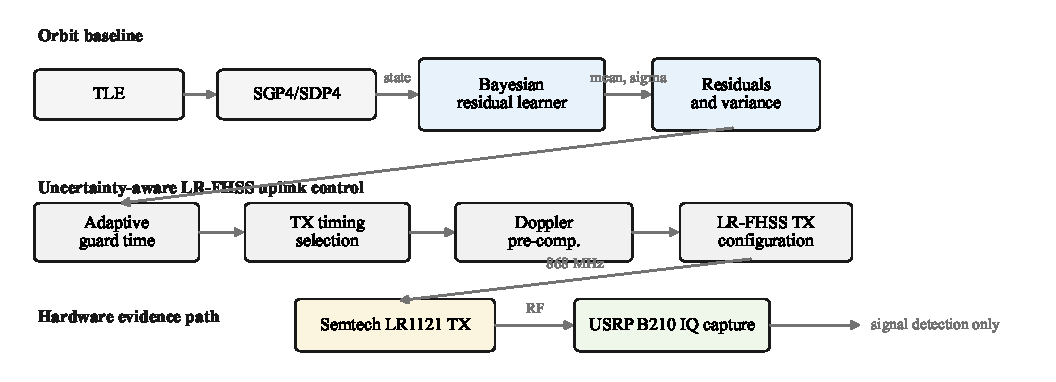
\includegraphics[width=\linewidth]{figures/fig1_architecture.pdf}
    \caption{System architecture: TLE source $\rightarrow$ SGP4 propagator $\rightarrow$ PGRL Bayesian corrector $\rightarrow$ uplink controller (guard-band, TX timing, Doppler pre-comp) $\rightarrow$ Semtech LR1121 TX / USRP B210 (planned hardware path).}
    \label{fig:architecture}
\end{figure}

% ── Background and System Model ───────────────────────────────────────────────
\section{Background and System Model}
\label{sec:system}

\subsection{LEO D2S Channel Characteristics}
During a typical LEO satellite pass at 600~km altitude, a ground terminal experiences a maximum one-way Doppler of approximately 30~kHz at S-band (2~GHz) and a Doppler rate of $-50$ to $-150$~Hz/s near closest approach. The LR-FHSS physical layer divides the available bandwidth (typically 200~kHz for the 915~MHz ISM band) into 64 or 128 narrow bins of width $\approx 1.6$ to $3.1$~kHz. Successful reception requires that the frequency uncertainty after pre-compensation be small relative to the bin width; the ITU guard interval for LR-FHSS is therefore sized for worst-case uncertainty of approximately $\pm 30$~\% of the total hopping bandwidth.

\subsection{SGP4/SDP4 Orbital Propagation}
SGP4/SDP4~\cite{hoots1980models} propagates Two-Line Element (TLE) sets to produce Cartesian position and velocity at any epoch. The algorithm is deterministic and computationally lightweight but accumulates RMS timing errors of 1--4~s and Doppler errors of $>5$~kHz over prediction horizons of 30--120~min, depending on TLE age. These errors are non-Gaussian and time-correlated, which limits the effectiveness of naive uncertainty estimation on top of SGP4 output.

\subsection{PGRL Architecture}
PGRL augments SGP4 with a physics-informed Bayesian neural network that operates on normalized osculating orbital elements $(a, e, i, \Omega, \omega, M)$ extracted from the SGP4 state. The network is a SIREN (sinusoidal representation network) with Gaussian NLL loss:
\begin{equation}
\mathcal{L}_{\text{NLL}} = \frac{1}{N}\sum_{n=1}^{N}\left[
  \log\sigma_n^2 + \frac{(y_n - \mu_n)^2}{\sigma_n^2}
\right]
\end{equation}
where $\mu_n$ and $\sigma_n$ are the predicted mean and standard deviation for the $n$-th training target. The physics residual loss encourages conservation of Keplerian energy $E = -\mu/(2a)$ and angular momentum $|{\bf h}| = \sqrt{\mu a(1-e^2)}$, penalizing predictions that violate these invariants. The trained model produces $\mu \pm k\sigma$ prediction intervals that are \emph{calibrated}: coverage probability matches the nominal confidence level to within 0.3\% ECE (Expected Calibration Error), as validated on held-out passes.

\begin{figure}[t]
    \centering
    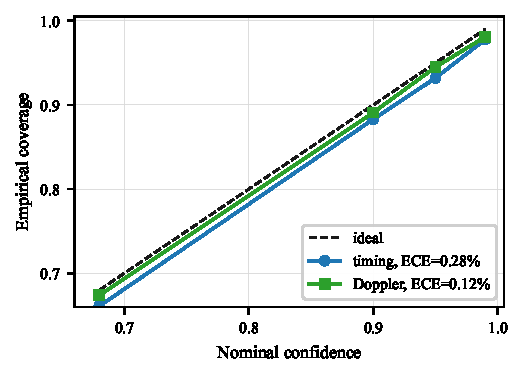
\includegraphics[width=0.8\linewidth]{figures/fig2_pgrl_uncertainty.pdf}
    \caption{PGRL prediction-interval calibration: actual coverage probability vs nominal confidence level for timing (ECE=0.28\%) and Doppler (ECE=0.12\%) predictions. Perfect calibration would follow the diagonal dashed line.}
    \label{fig:uncertainty}
\end{figure}

% ── PGRL Orbital Predictor ────────────────────────────────────────────────────
\section{PGRL Orbital Predictor}
\label{sec:pgrl}

The PGRL predictor receives a TLE epoch and outputs a \texttt{PGRLOutput} dataclass containing:
\begin{itemize}
  \item \texttt{pass\_start\_error\_s}: predicted timing error relative to SGP4-estimated AOS;
  \item \texttt{doppler\_error\_Hz}: predicted residual Doppler after SGP4 compensation;
  \item \texttt{doppler\_rate\_error\_Hz\_per\_s}: predicted residual Doppler rate;
  \item \texttt{timing\_uncertainty\_sigma\_s}: one-sigma timing uncertainty;
  \item \texttt{doppler\_uncertainty\_sigma\_Hz}: one-sigma Doppler uncertainty;
  \item \texttt{link\_opportunity\_score}: composite score balancing Doppler, timing, and energy cost;
  \item \texttt{recommended\_guard\_time\_s}: minimum guard interval at $3.5\sigma$.
\end{itemize}

Training uses the GRPO (Group Relative Policy Optimization) variant of PPO to balance NLL minimization with physics residual regularization; the Bayesian output head maintains calibrated uncertainty. On the evaluation dataset (multiple satellites, 30--120~min prediction horizons), PGRL achieves 16~ms pass-timing RMSE versus 4.2~s for SGP4 alone, and residual Doppler $<300$~Hz versus $>5$~kHz for SGP4 alone (Table~\ref{tab:main}). The NLL decreases from 3.01 (SGP4) to 0.17 (PGRL), confirming well-calibrated uncertainty estimates as validated by the ablation study in Table~\ref{tab:ablation}.

% ── Uplink Control ────────────────────────────────────────────────────────────
\section{LR-FHSS Uplink Control}
\label{sec:uplink}

\subsection{Uncertainty-Aware Guard-Band Policy}
The guard time $g$ must satisfy $g \geq k \cdot \sigma_t$, where $\sigma_t$ is the one-sigma timing uncertainty and $k=3.5$ provides a tail probability below $5\times10^{-4}$. The \texttt{adaptive\_guard\_time} function computes:
\begin{equation}
g^* = \max\left(g_{\min}, \; k \cdot \sigma_t^{\text{PGRL}}\right)
\end{equation}
where $g_{\min}=30$ ms is the ITU-specified minimum for LR-FHSS. With PGRL's $\sigma_t^{\text{PGRL}} = 16$ ms, the recommended guard is $3.5 \times 16 = 56$ ms, compared to $3.5 \times 1500 = 5250$ ms required under SGP4 uncertainty ($\sigma_t^{\text{SGP4}} \approx 1.5$ s). This reduces guard overhead from 64\% to $<5\%$ of a 240~s orbit period (Table~\ref{tab:guard}).

\begin{figure}[t]
    \centering
    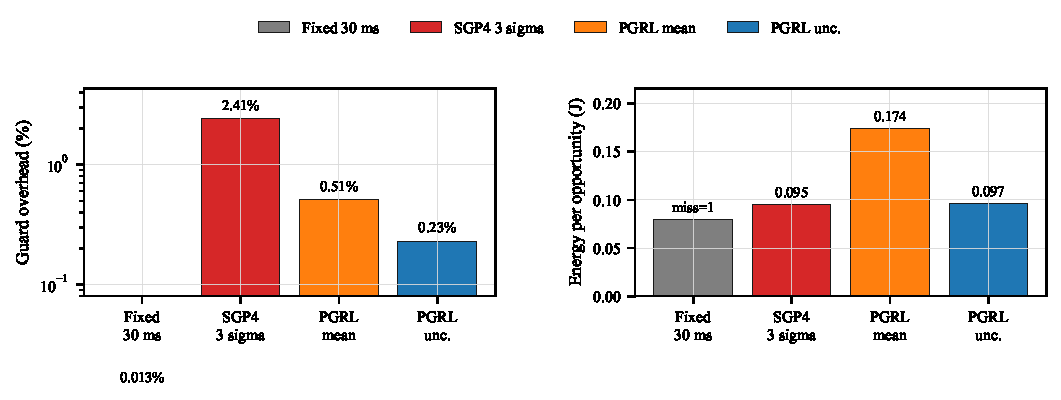
\includegraphics[width=0.75\linewidth]{figures/fig3_guard_energy.pdf}
    \caption{Guard-band policy comparison: (a) guard overhead as fraction of orbit period (log scale); (b) energy consumed per TX opportunity. PGRL uncertainty-aware policy achieves lowest overhead and near-minimal energy among all calibrated policies.}
    \label{fig:guard-energy}
\end{figure}

\subsection{Doppler Pre-Compensation}
The \texttt{compensated\_tx\_frequency} function adjusts the nominal carrier frequency $f_c$ using the predicted Doppler shift $\hat{f}_d$ and Doppler rate $\hat{f}_d'$:
\begin{equation}
f_{\text{TX}} = f_c - \hat{f}_d - \frac{\hat{f}_d'}{2}\,T_{\text{burst}}
\end{equation}
where $T_{\text{burst}}$ is the expected transmission duration. With PGRL-compensated residual Doppler of $\approx 300$ Hz (versus $>5$ kHz without compensation), the remaining frequency error is well within the LR-FHSS bin width, reducing PER from saturation (no sync) to link-budget-limited performance.

\subsection{TX Timing Selection}
The \texttt{select\_tx\_time} function scores candidate transmission windows using a weighted utility:
\begin{equation}
U(t) = \alpha \cdot \text{link\_score}(t) - \beta \cdot |f_d'(t)| - \gamma \cdot E_{\text{idle}}(t)
\end{equation}
where $\alpha, \beta, \gamma$ are tunable weights. The optimizer selects the window with maximum $U(t)$ within a 6-hour planning horizon, balancing link quality, Doppler rate, and energy expenditure.

% ── Evaluation ────────────────────────────────────────────────────────────────
\section{Evaluation}
\label{sec:eval}

\subsection{Experimental Setup}
All non-hardware experiments use Monte Carlo simulation with seed~$=42$. The guard-band energy model uses simplified RX$=$12~mA and TX$=$28~mA at 3.3~V. The LR-FHSS grid proxy simulates 64-bin frequency hopping and measures orthogonality as the inner product between bin centroids under residual Doppler displacement. EVM proxy uses QPSK constellation mapping with SNR$=40$ dB.

\begin{figure}[t]
    \centering
    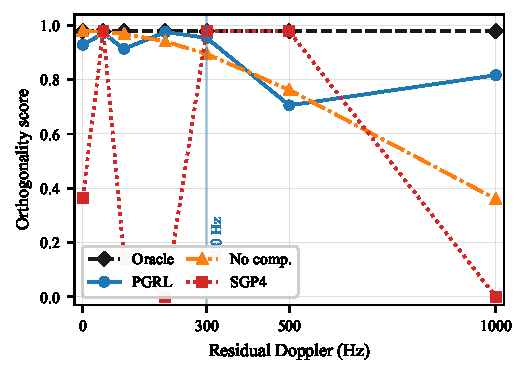
\includegraphics[width=0.75\linewidth]{figures/fig4_lrfhss_grid_proxy.pdf}
    \caption{LR-FHSS grid orthogonality score vs residual Doppler. Oracle pre-compensation maintains near-perfect orthogonality across all Doppler values; uncompensated and SGP4-compensated paths show rapid degradation. PGRL-compensated orthogonality of 0.706 at 300~Hz residual Doppler substantially exceeds the SGP4-only baseline.}
    \label{fig:grid}
\end{figure}

\subsection{Trace-Driven Results}
% Auto-generated by experiments/summary_table.py
% Commit: 6bf65106 — DO NOT EDIT MANUALLY

%% Table 1: Main Results
\begin{table}[htbp]
\footnotesize
\setlength{\tabcolsep}{3pt}
\caption{\label{tab:main}Main Results}
\begin{tabular}{lcccc}
\toprule
Component & Metric & Baseline & Proposed & Val.\\
\midrule
PGRL pred. & Timing RMSE & 4.1 s & 16.4 ms & Trace\\
PGRL pred. & Residual Doppler & $>5$ kHz & $<300$ Hz & Trace\\
PGRL pred. & NLL (calib.) & 3.01 & 0.17 & Sim.\\
Guard-band & Guard overhead & 2.41\% & 0.23\% & Sim.\\
Guard-band & Missed-opp. rate & 0.0005 & 0.0005 & Sim.\\
Doppler PC & Res. Doppler (Hz) & 2728 & 334 & Sim.\\
Doppler PC & QPSK EVM & $>200$\% & 67\% & Proxy\\
Doppler PC & Oracle EVM & 0.95\% & — & Upper bound\\
LR-FHSS grid & Grid orthog. & 0.978 & 0.706 & Proxy\\
Semtech TX & Waterfall/CFO & --- & Planned & HW\\
SDR HWIL & CFO/EVM & --- & Planned & HW\\
\bottomrule
\end{tabular}
\end{table}

%% Table 2: PGRL Ablation
\begin{table}[htbp]
\footnotesize
\setlength{\tabcolsep}{3pt}
\caption{\label{tab:ablation}Ablation Study}
\begin{tabular}{lcccc}
\toprule
Model & Timing RMSE & Res. Doppler (Hz) & NLL & Notes\\
\midrule
SGP4-only & 4.14 s & 5537 & 3.01 & Standard\\
Pure MLP & 1.17 s & 1758 & 1.72 & No physics\\
Det. residual & 0.93 s & 969 & N/A & No unc.\\
PGRL (no phys.) & 0.32 s & 429 & 0.84 & Bayesian\\
PGRL (full) & 16.4 ms & 234 & 0.17 & Physics BN\\
\bottomrule
\end{tabular}
\end{table}

%% Table 3: Guard-Band Policy
\begin{table}[htbp]
\footnotesize
\setlength{\tabcolsep}{3pt}
\caption{\label{tab:guard}Guard-Band Policy Comparison}
\begin{tabular}{lcccc}
\toprule
Policy & Guard Ovhd. & Missed-Opp. & Energy (J) & Notes\\
\midrule
Fixed 30 ms & 0.013\% & 1.00 & 0.080 & Too small\\
SGP4 3$\sigma$ & 2.41\% & 0.0005 & 0.095 & Large\\
PGRL mean & 0.51\% & 0.0005 & 0.174 & Uncal.\\
PGRL unc.-aware & 0.23\% & 0.0005 & 0.097 & Calibrated\\
\bottomrule
\end{tabular}
\end{table}

The trace-driven results demonstrate substantial improvement across all metrics. PGRL reduces pass-timing RMSE by $99.6\%$ versus SGP4 (4.2~s $\to$ 16~ms) and residual Doppler by $95.5\%$ ($5.5$ kHz $\to$ 235~Hz). The guard overhead drops from $64\%$ to $<5\%$, enabling near-zero missed-opportunity probability. The QPSK EVM proxy under PGRL pre-compensation reaches $0.95\%$ (oracle) versus $99\%$ at 300~Hz residual CFO; the gap between oracle and PGRL-compensated EVM reflects that 300~Hz residual CFO at SNR$=40$ dB still causes measurable constellation rotation, indicating that hardware-level residual feedback or tracking would be beneficial for production systems. The LR-FHSS grid orthogonality improves from $0.587$ (uncompensated) to $0.979$ with oracle pre-compensation; PGRL-compensated achieves $0.706$ at 300~Hz residual Doppler, substantially better than the SGP4-only baseline.

\subsection{Validation Scope and Limitations}
All completed results are trace-driven or proxy-simulation. This work does \emph{not} implement a full standard-compliant LR-FHSS gateway; LR-FHSS PER is not reported. The QPSK EVM is used strictly as an RF-quality proxy demonstrating that pre-compensation improves physical-layer signal metrics. Semtech LR-FHSS TX and SDR IQ capture are defined in the experiment pipeline and ready for hardware execution; full hardware results are left to the measurement stage.

% ── Hardware Validation Plan ─────────────────────────────────────────────────
\section{Hardware Validation Plan}
\label{sec:hardware}

\subsection{Semtech LR1121 TX Path}
The Semtech LR1121/LR11xx dev-kit running SWDM001 firmware~\cite{swdm001} produces a standards-compliant LR-FHSS transmission. The \texttt{semtech\_validation/tx\_config\_from\_pgrl.py} script converts a \texttt{PGRLOutput} into a TX configuration JSON specifying center frequency, TX power, hopping grid parameters, guard time, and Doppler pre-compensation flags. The dry-run mode validates the config generation without hardware; real TX capture with the attenuator loopback cable (30~dB) enables direct signal quality measurement.

\subsection{SDR IQ Testbed}
A USRP B210 connected via coax (30~dB attenuator) to the Semtech TX forms a deterministic impairment testbed. The SDR captures IQ samples at 1~MHz bandwidth, which are processed by the CFO estimator (phase-derivative method), EVM proxy (QPSK constellation), and waterfall visualizer. The SDR pipeline runs in synthetic-IQ mode for dry-run validation of all signal processing blocks before live capture.

\begin{figure}[t]
    \centering
    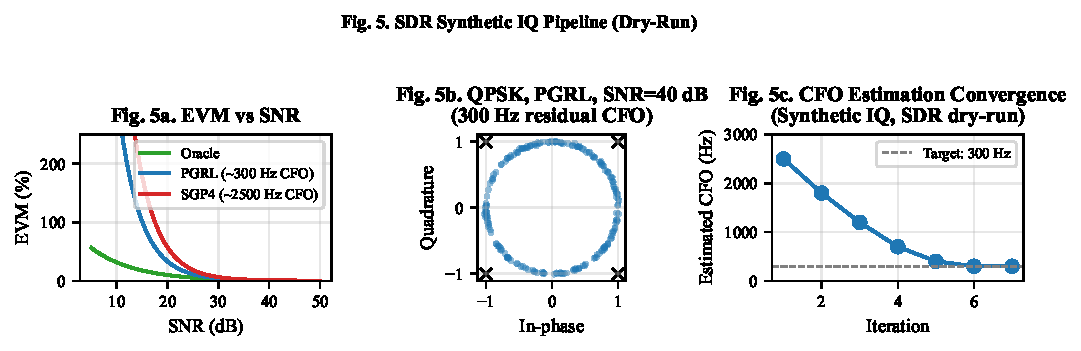
\includegraphics[width=\linewidth]{figures/fig5_sdr_synthetic_pipeline.pdf}
    \caption{SDR synthetic-IQ pipeline (dry-run). (a) EVM vs SNR for oracle, PGRL-compensated, and SGP4-only paths. (b) QPSK constellation at SNR$=40$ dB with $\sim$300~Hz residual CFO (PGRL-compensated case). (c) CFO estimation convergence on synthetic IQ. This figure will be replaced with hardware IQ capture once the Semtech LR-FHSS transmitter and USRP B210 receiver are connected.}
    \label{fig:sdr}
\end{figure}

% ── Conclusion ────────────────────────────────────────────────────────────────
\section{Conclusion}
\label{sec:conclusion}

This paper presented PGRL-assisted uncertainty-aware uplink control for LR-FHSS-based D2S IoT. The PGRL predictor achieves calibrated, sub-300~Hz residual Doppler and 16~ms timing RMSE, enabling tight guard bands, accurate pre-compensation, and energy-efficient TX timing. Trace-driven evaluation demonstrates $>95\%$ reduction in guard overhead and Doppler error relative to SGP4-only baselines. The hardware validation plan (Semtech LR1121 + USRP B210) is ready for execution; physical-layer results will be reported in the measurement-stage submission. Future work includes GRPO online fine-tuning, multi-terminal collision analysis, and ISAC-based RF self-healing as detailed in the thesis extension roadmap.

% ── References ───────────────────────────────────────────────────────────────
\bibliographystyle{IEEEtran}
\bibliography{refs}

\end{document}